\newpage
\section{Materials and methods}\label{sec:matandmet}

This section will go through the structure of the dataset, the model used in the experiments for classifying and the structure of the experiments that was done.

\subsection{Dataset description}

As mentioned earlier the dataset was collected for the study in~\cite{original_study}. There was collected ECG-data from 298 patients, and these were sorted into the five categories described in section~\ref{subsec:heartrhythm}. There are two different datasets within the data, one with compressions and one without. The dataset without compressions is called "Clean Cuts" and has 2833 cuts of ECG-data that was used for this project.  The raw data was sampled at 500~Hz and with 16 bit resolution. For this project only the "Clean Cuts" dataset was used.

Figure \ref{fig:ecg_signals} shows three samples from each category, where each cut spans four seconds.  As seen the amplitude is different between the classes and therefore the samples were not normalized.

\begin{figure}[H]
    \foreach \v in {VF, VT, AS, PEA, PGR} {
        \begin{minipage}[b]{0.49\textwidth}
            \includesvg[width=1\textwidth]{Img/dataset/\v.svg}
            \vspace{-0.5cm}
            \caption*{\v}
        \end{minipage}
    }
    \caption{Three samples of the ECG signal for each category.}
    \label{fig:ecg_signals}
\end{figure}

Figure \ref{fig:n_labels} shows how many samples there are per category. It shows that the dataset is not balanced, as the biggest category, PEA (912 samples), has over 5 times as many samples as the smallest category, VT (166 samples). Because of this, balanced accuracy was used to evaluate the models instead of normal accuracy. This is described more in subsection~\ref{subsec:experiments}.

\begin{figure}[H]
    \centering
    \includesvg[width=0.6\textwidth]{Img/dataset/samples_per_label.svg}
    \caption{Number of samples per category in the dataset.} 
    \label{fig:n_labels}
\end{figure}

\subsection{Dataset partitioning}
The dataset was divided into training, validation and test-sets, first with $90\%$ in the training set and $10\%$ in the test set. Then the training set is split into ten folds using stratified k-fold cross validation to get validation and test data. The fact that it is stratified means that the ten folds has the same class distribution as the original dataset. For each trial, the weights in the model that gives the lowest validation loss will be saved and used to test against the test set.


\subsection{Model architecture}\label{subsec:modelarch}
% Things to explain:\\
% -General structure: We used the same as last year and improved it with implementation as \cite{2020} did.\\
% -Activation\\
% -Pooling or stride. Maxpooling and global maxpooling.\\
% - Batch normalization\\
% -layers and filter size\\
% -Kernel size\\
% -Padding?\\
% -Dropout\\
% -Modular design?\\

Last years project, which was used as a starting point this year, tried out different structured models to find the one that worked best for classifying hearth rhythms~\cite{cardiac}. This year, there was more focus on trying out different parameters for one general structure, and this was inspired by the article~\cite{2020}. 

The CNN model is illustrated in figure~\ref{fig:CNN_model}. After the input layer there was implemented N convolutional blocks, where N is a tuneable parameter. Inside this convolutional block there are four different types of layers: 1D convolution, batch normalization, max pooling and a dropout layer. One-dimensional convolutional layers and max-pooling are both explained in subsection~\ref{subsec:CNNtheory}. The main purpose of the convolutional layer is to let the model learn some important features of the input data, while max-pooling decreases the spatial dimensions of the feature map.

Batch normalization is a technique used to normalize the inputs of a layer in a neural network. The main purpose of batch normalization is to improve optimization, and it helps to stabilize and accelerate the training process~\cite{deeplearning}. Lastly in this block there is a dropout layer. The purpose of a dropout layer is to prevent overfitting in the network. It chooses random neurons and sets them to zero with a certain probability.

All the layers in the model, except the output layer, uses the same activation function: Rectified Linear Unit (ReLU). ReLU has become the default activation function for CNNs, because of the good performance it achieves~\cite{ReLU}. The output ReLU activation function is either directly the input if it is positive, and otherwise it is zero.

After the N convolutional blocks there comes a one-dimensional max-pooling layer, and then two dense layers. All these layers use ReLU as an activation function. The global max-pooling layer moves a window over the input, and outputs the maximum value for each window position. In a dense layer, all the inputs are connected to all the outputs, or in other words: the layer is fully connected. 

Lastly comes the fully connected output layer, where the hearth rhythm is classified into one of the five hearth rhythms. Here the activation function that is used is called softmax. This activation function scales the output numbers into probabilities. This makes the output the probability for the heart rhythm to belong to the class. 

\begin{figure}[H]
    \centering
    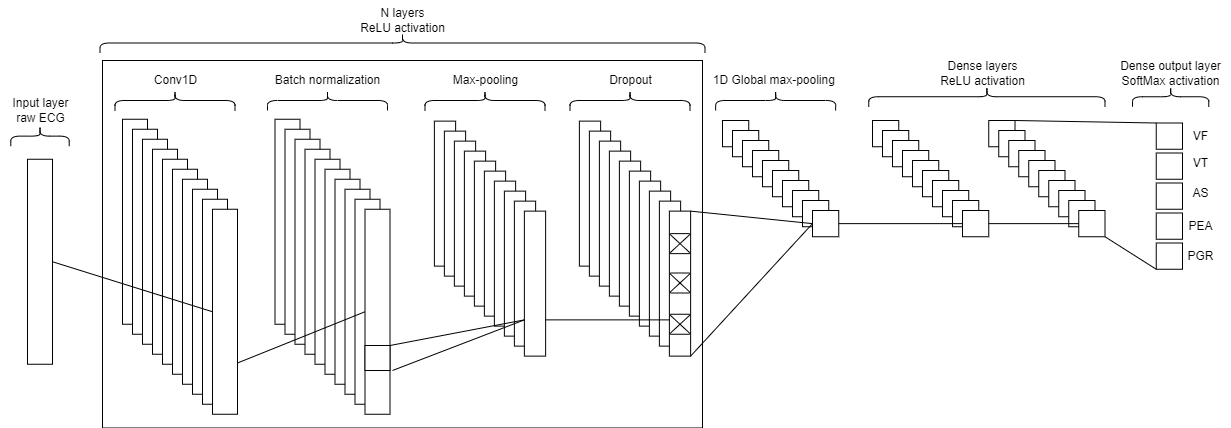
\includegraphics[width=1\linewidth]{Img/CNN_rhythm_classify.png}
    \caption{The structure of the CNN model.}
    \label{fig:CNN_model}
\end{figure}

\subsection{Experiments}\label{subsec:experiments}
When testing the model some of the parameters were set to a fixed value. The batch size was set to 32, learning rate was set to 0.001 and there was a maximum of 250 epochs, with early stopping if the validation loss did not improve for 30 epochs. Additionally the number of fully connected hidden layers was set to two (as described in subsection~\ref{subsec:modelarch}), and the downsampling was done with the pool size set to two.

To test the effect of the different hyperparameters \textit{Keras Tuner} was used to perform random search~\cite{omalley2019kerastuner}. Keras Tuner is a framework with algorithms to find the best parameters for a model. For each N there was done 250 trials, with 10-fold cross validation in each trial. Every trial consist of randomly selected parameters. The parameters which were experimented with are listed below, with $i = 1,2,..,N$ and $j = 1,2$.

\begin{itemize}
    \item N = [2, 3, 4, 5], layers of convolutional blocks in the model.
    \item Dropout: [0.1, 0.2, .., 0.9]
    \item $K_i$ = [5, 10, 15, 20, 25, 30, 40, 50], kernel sizes in Conv1D
    \item $F_i$ = [5, 10, 15, 20, 25, 30, 40, 50], number of filters in Conv1D
    \item $FC_j$ = [16, 32, 64, 128], number of nodes in the fully connected hidden layers 
\end{itemize}

We used Balanced Accuracy (BAC) as our criteria to evaluate the models since the dataset is very unbalanced. Balanced accuracy is a development of the normal accuracy, instead of looking at only how many of the predictions that are correct it looks at how many are correct for each class. This means that it is more accurate for imbalanced datasets~\cite{accuracy}.

$$
\text{BAC} = \frac{\text{Sensitivity} + \text{Specificity}}{2}
$$

After the initial experiments, the dropout and $FC_j$ was fixed, and more experiments were carried out while varying $F_i$ and $K_i$. This time there was done 400 trials for each N.